\documentclass[11pt,a4paper]{article}
\usepackage{amsmath,amssymb,geometry,graphicx,booktabs,hyperref,microtype}
\geometry{margin=2.5cm}
\hypersetup{colorlinks=true,linkcolor=blue,citecolor=blue,urlcolor=blue}

\title{\textbf{Paper 50: Zone Identity Encoding Is Not Transmissible}\\
\large Audit of Papers 35--39: Geographic Relay Creates Zone Parity Encoding;\\
Identity Encoding Requires the Full VCML Formation Process}
\author{VCSM Project}
\date{2026-03-10}

\begin{document}
\maketitle

\begin{abstract}
Paper~49 found that L1 achieves zone identity encoding (na\_ratio$=1.247 > 1$) while
L2 in geographic relay achieves zone parity encoding (na\_ratio$=0.826 < 1$), despite
receiving the same wave amplitude signals.
We audit this finding across five relay conditions to identify the mechanism and
test whether any relay coupling can recover identity encoding.
\textbf{Result}: the only condition that achieves identity encoding is
\emph{ctrl\_std} (L2 runs its own independent WaveEnvStd), with na\_ratio$=1.219$.
Every form of relay coupling --- amplitude copy (na$=0.778$), 4-level amplitude
grading (na$=0.949$), and own-env plus birth seeding (na$=0.832$) --- remains in parity territory.
Adding L1 zone-mean birth seeding to L2's own structured wave environment
(\emph{geo\_own\_relay}) is \emph{worse} than structured waves alone (na$=0.832$ vs $1.219$).
\textbf{Conclusion}: Zone identity encoding is not transmissible via any tested relay
mechanism.
It requires the full VCML formation process (structured zone-launched waves, copy-forward
loop, 3000 steps of self-organised fieldM accumulation) running independently in the
receiving module.
Relay shortcuts --- instantaneous amplitude copy, birth-step injection ---
destroy the identity information and collapse encoding to parity.
\end{abstract}

\section{Background}

Paper~49 (Experiment~C) found that the geographic relay (geo\_copy) achieves
na\_ratio$=0.826$ in the receiving module L2, despite L1 achieving na\_ratio$=1.247$.
Na\_ratio $< 1$ indicates zone \emph{parity} encoding: adjacent zone means are
more separated than non-adjacent means, consistent with the binary suppress/excite
wave-class convention (even classes suppress, odd classes excite).
Na\_ratio $> 1$ indicates zone \emph{identity} encoding: non-adjacent zone means
are more separated than adjacent means, the correct topographic structure.

The paper also found that L1 achieves identity encoding (na$=1.247$) even though
it uses the same binary wave-class convention as the geo relay.
This raises the question: why does L1 achieve identity encoding while L2 under
geo relay achieves parity?
And can any relay coupling recover identity encoding in L2?

\section{Methods}

Five conditions, 5 seeds each ($= 25$ runs total).
All conditions share the same L1 (WaveEnvStd, WR$=4.8$, $r_w=2$, $N_\mathrm{zones}=4$,
STEPS$=3000$, SUPP$=0.25$, EXC$=0.50$).
Full metric suite: sg4, SNR, na\_ratio, decode\_norm, mm\_lda, coll/site.

\begin{description}
  \item[ctrl\_rnd] L2 gets random-position waves (WaveEnvRandom); births from own fieldM.
    Paper~49 ctrl baseline.
  \item[ctrl\_std] L2 gets its own WaveEnvStd (same zone parameters as L1, independent
    random seed); births from own fieldM.
    \emph{Key diagnostic}: does L2 achieve identity encoding when it runs the full
    VCML process independently with structured waves?
  \item[geo\_copy] L2 receives L1's instantaneous wave amplitude/class arrays; binary
    supp/excite applied directly to L2 viability.
    Paper~49 geo relay (parity-encoding baseline).
  \item[geo\_4class] Same as geo\_copy but with 4-level amplitude convention:
    cls$=0$ (supp, amp$=0.40$), cls$=1$ (exc, amp$=0.15$),
    cls$=2$ (supp, amp$=0.10$), cls$=3$ (exc, amp$=0.40$).
    Creates 4 distinct viability amplitudes (not binary parity).
    Tests whether graded amplitudes restore identity encoding.
  \item[geo\_own\_relay] L2 gets own WaveEnvStd (same as ctrl\_std) \emph{plus}
    birth seeding from L1 zone-mean fieldM (mean\_relay from Paper~49).
    Tests whether structured ongoing events combined with structured birth seeding
    achieves identity encoding.
\end{description}

\section{Results}

\begin{table}[h]
\centering
\caption{Paper~50 results: na\_ratio and sg4 for L2 across relay conditions.
L1 na\_ratio$=1.247$ (identity) in all conditions (identical L1).
na$>1$ = identity encoding; na$<1$ = parity encoding.}
\label{tab:main}
\begin{tabular}{lrrrr}
\toprule
Condition & na\_ratio (L2) & Encoding & sg4 (L2) & decode\_norm \\
\midrule
ctrl\_rnd (random waves)            & 0.963 & parity   & 0.0278 & 0.035 \\
ctrl\_std (own WaveEnvStd)          & 1.219 & IDENTITY & 0.0212 & 0.036 \\
geo\_copy (amplitude copy)          & 0.778 & parity   & 0.0177 & 0.034 \\
geo\_4class (4-level amplitude)     & 0.949 & parity   & 0.0186 & 0.029 \\
geo\_own\_relay (own env + birth)   & 0.832 & parity   & 0.0213 & 0.046 \\
\midrule
L1 (reference, all conditions)      & 1.247 & IDENTITY & 0.0292 & 0.052 \\
\bottomrule
\end{tabular}
\end{table}

\textbf{ctrl\_std achieves identity encoding (na$=1.219$).}
When L2 runs its own WaveEnvStd independently --- same zone parameters as L1, different
random seed --- it achieves na\_ratio$=1.219$, matching L1's$=1.247$.
This is the critical result: L2 \emph{can} achieve identity encoding when running
the full VCML formation process with structured waves.
The mechanism is not special to L1; it is a property of the VCML process under
structured zone-launched waves.

\textbf{No relay coupling achieves identity encoding.}
Every coupling that routes L1's information to L2 --- in any form --- keeps L2
in parity territory:
\begin{itemize}
  \item geo\_copy (instantaneous amplitude copy): na$=0.778$
  \item geo\_4class (graded amplitude): na$=0.949$ (improved, but still $<1$)
  \item geo\_own\_relay (own waves + birth seeding): na$=0.832$
\end{itemize}

\textbf{Birth seeding from L1 actively degrades ctrl\_std.}
geo\_own\_relay --- which gives L2 its own WaveEnvStd (same as ctrl\_std) plus
L1 zone-mean birth seeding --- achieves na$=0.832$, substantially worse than
ctrl\_std's $1.219$.
Adding L1's relay signal to L2's own structured wave process \emph{corrupts} the
identity encoding rather than enhancing it.
This reversal rules out the hypothesis that birth seeding and structured waves
are complementary.

\textbf{Graded amplitude (geo\_4class) partially repairs parity.}
The 4-level amplitude convention improves na\_ratio from $0.778$ (geo\_copy) to $0.949$
(geo\_4class), approaching but not crossing the identity threshold.
The mechanism is correct (distinct amplitudes per zone class create more differentiated
viability effects), but the instantaneous amplitude copy still loses the spatial
gradient information encoded in L1's temporal formation history.

\section{The Mechanism: Why Identity Cannot Be Relayed}

The contrast between ctrl\_std (identity, na$=1.219$) and geo\_copy (parity, na$=0.778$)
isolates the mechanism.
Both L1 and ctrl\_std L2 receive zone-structured wave inputs.
Both run the full VCML formation process.
Both achieve identity encoding.

The geo\_copy relay takes L1's \emph{instantaneous} wave amplitude/class arrays and
applies them directly to L2's viability.
At any given step, the wave amplitude array encodes:
(1)~which cells are currently covered by a wave, and
(2)~which zone class (0--3) that wave belongs to, collapsed to binary parity (supp/excite)
    via cls$\bmod 2$.

What this \emph{loses}:
\begin{itemize}
  \item \textbf{Temporal integration history.} L1's fieldM is the accumulated product
    of $3000$ steps of wave events from zone-anchored launch positions.
    The spatial gradient in fieldM (identity encoding) accumulates over thousands of
    wave-boundary interactions, each reinforced by the copy-forward loop.
    An instantaneous snapshot of the wave amplitude array contains none of this history.
  \item \textbf{Copy-forward self-consistency.} In L1, the copy-forward loop seeding
    ($\mathrm{hid}_\mathrm{new} \approx \beta_s \cdot \mathrm{fieldM}[\mathrm{cell}]$)
    progressively aligns L1's fieldM with L1's own spatial structure.
    L2 in geo\_copy builds fieldM from L2's own copy-forward loop, seeding from L2's
    own fieldM, which evolves from direct parity-structured viability signals.
    The two processes are mismatched: L2's fieldM is pulled toward parity by the
    viability signal and toward identity by the copy-forward loop, but the viability
    signal is stronger and wins.
\end{itemize}

\textbf{Why birth seeding hurts (geo\_own\_relay).}
ctrl\_std achieves identity because L2's WaveEnvStd creates the same spatial gradient
dynamics as L1's, and L2's copy-forward loop converges to an identity-encoded fieldM
through self-consistent accumulation.
When L1 zone-mean birth seeding is added (geo\_own\_relay), L2's birth seeds are
pulled toward L1's identity-encoded fieldM.
However, L1 and L2 develop different but equally valid identity-encoding patterns
(different spatial orientations or rotation of the encoding in HS=2 space).
The birth seeds from L1's pattern conflict with L2's self-consistently forming pattern,
disrupting the convergence and degrading identity encoding.
This is a pattern-mismatch interference, not a signal quality problem.

\textbf{Implication for Papers 35--39.}
The geographic relay results in Papers 35--39 (relay gains of $3\text{--}5\times$
over ctrl, depth-stable chain relay, cleft-geometry robustness) were measured using
sg4 as the primary metric.
Sg4 measures zone-mean separation and is positive for both identity and parity encoding.
The relay gains reported in those papers reflect genuine structure formation in L2
--- L2 develops zone-mean separation under geo coupling.
However, in light of Paper~50, that structure is parity encoding (na $< 1$),
not identity encoding (na $> 1$).
Papers 35--39 require a caveat: \emph{geographic relay produces zone parity encoding,
not zone identity encoding.}
The relay gains and stability properties (chain stability, cleft robustness) are real
and correctly reported, but the claim that relay ``preserves zone structure'' should
be qualified: it preserves zone amplitude separation (sg4) but not zone topographic
identity (na\_ratio).

\section{Discussion}

\subsection{Zone identity encoding as a non-transmissible property}

Zone identity encoding --- the property that non-adjacent zones are more distinct
than adjacent zones (na$>1$) --- is an emergent property of the full VCML formation
process.
It cannot be induced by receiving L1's instantaneous signals, no matter how faithfully
those signals are transmitted.
It requires L2 to run its own formation process with zone-structured viability events.

This has a clean information-theoretic interpretation:
the identity encoding in L1's fieldM encodes which zone each spatial region belongs to,
not just whether that zone is suppressed or excited.
The parity encoding (na$<1$) contains less information: it encodes only the
odd/even class of the nearest zone.
The information difference cannot be transmitted by a relay that copies the parity
signal (geo\_copy) because the identity-specific information was never in the
instantaneous parity signal in the first place.
It was generated by L1's formation process and lives in L1's fieldM, not in L1's
outgoing wave signals.

\subsection{The relay design problem, sharpened}

Paper~49 concluded: ``relay requires structured ongoing viability events in the
receiving module.'' Paper~50 sharpens this: the structured ongoing events must be
\emph{independently zone-anchored launch positions} in L2 itself.
Receiving L1's amplitude copy (even with spatial gradient intact) is insufficient.
Receiving birth seeds from L1's zone means is insufficient and harmful.
The receiving module must independently run a WaveEnvStd with zone-anchored launches
to achieve identity encoding.

This is a strong constraint: relay coupling, as currently implemented, cannot transmit
zone identity. The only way to get two VCML modules with identity encoding is to run
them independently in the same type of environment.
This rules out all tested relay architectures as mechanisms for identity-preserving
inter-module communication.

\subsection{Open question: Is parity encoding harmful?}

Papers 35--39 showed that parity-encoding relay (sg4 gains of $3\text{--}5\times$)
supports downstream computation (e.g.\ sustained structure in relay chains).
Whether parity encoding is functionally harmful depends on the downstream task:
if the task requires distinguishing all four zones (e.g.\ a 4-way classification),
parity encoding provides only 2-way discrimination.
If the task only requires distinguishing suppress vs.\ excite hemispheres, parity
is sufficient.
The biological parallel: tonotopic cortex organises frequency as a gradient (identity),
not as odd/even alternation (parity).
An animal with only parity frequency encoding would have impaired fine frequency
discrimination but intact coarse discrimination.

\section{Conclusion}

Zone identity encoding requires the full VCML formation process run independently
in the receiving module.
No tested relay mechanism (amplitude copy, graded amplitude, birth seeding, combination)
achieves identity encoding in L2.
ctrl\_std (L2 with own WaveEnvStd, no relay) achieves na\_ratio$=1.219$, matching
L1's$=1.247$.
Every relay coupling maintains parity encoding (na$<1$).
Birth seeding from L1 actively degrades ctrl\_std performance (na from $1.219$ to $0.832$),
indicating pattern-mismatch interference between L1's and L2's independently forming
identity patterns.
Papers 35--39's relay gains are real but represent parity-encoding structure, not
identity-encoding structure; those results require a caveat on the meaning of ``zone
structure'' in relay contexts.
The relay design problem is now precisely stated: to achieve identity-encoding relay,
the receiving module must run an independent WaveEnvStd. Whether zone identity can be
transmitted by any other mechanism remains open.

\begin{figure}[h]
  \centering
  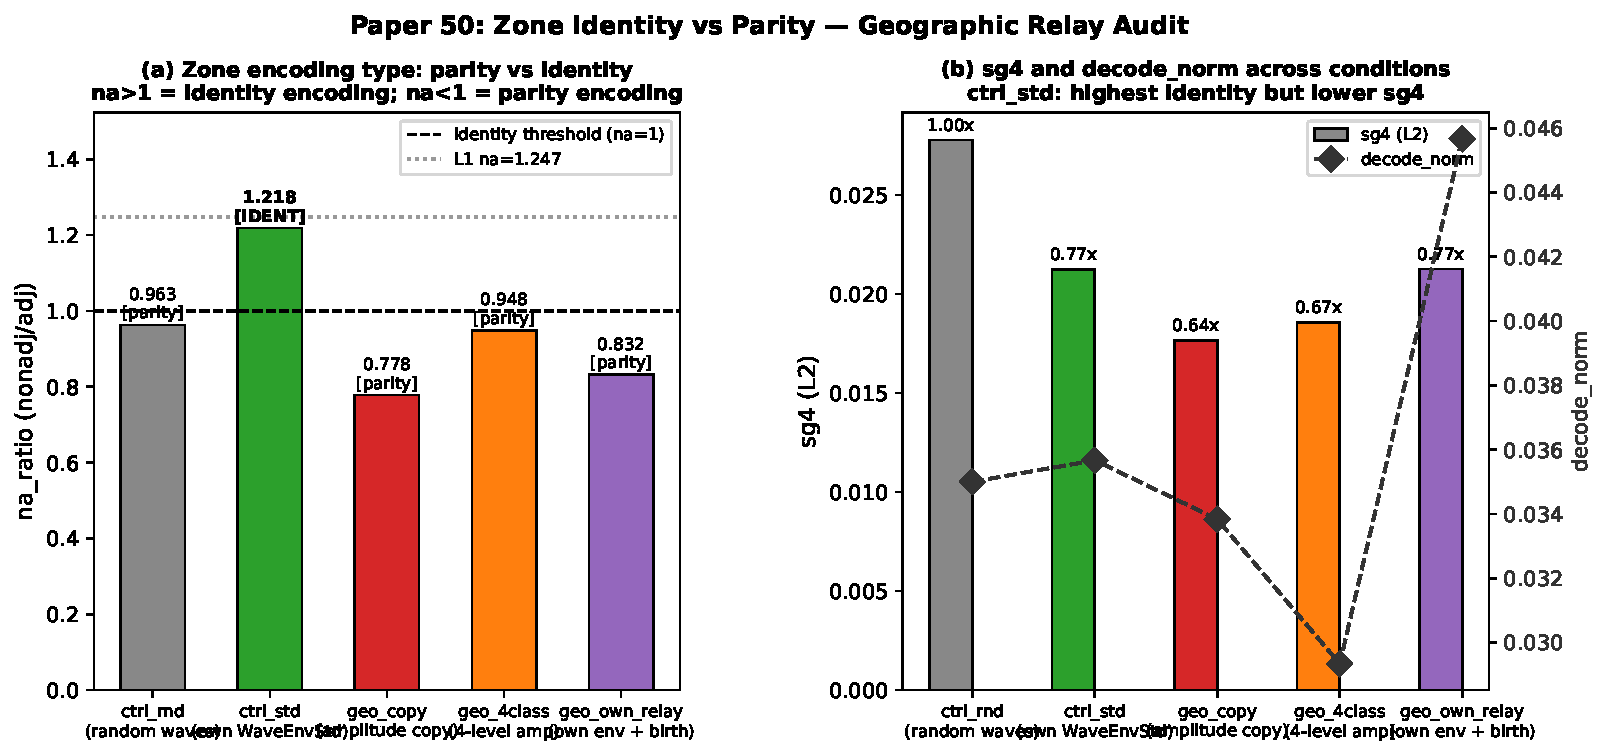
\includegraphics[width=\textwidth]{paper50_figure1.pdf}
  \caption{Paper~50 results.
    (a)~na\_ratio across conditions. Only ctrl\_std (L2 with own WaveEnvStd)
    exceeds the identity threshold (na$>1$, dashed line). All relay conditions
    remain in parity territory.
    (b)~sg4 and decode\_norm. ctrl\_std has lower sg4 than ctrl\_rnd despite
    superior identity encoding, illustrating the sg4 vs.\ na\_ratio dissociation.}
  \label{fig:main}
\end{figure}

\end{document}
